%% =============================
%%      IMPORTANTE
%% ESTE ARQUIVO DEVE ESTAR SALVO COMO
%%      UTF - 8
%% =============================

% ----------------------------------------------------------
% Este capítulo é parte integrante do arquivo mestre
% Relatorio_TCC_Mestrado_Base_VERSÃO_SUBVERSÃO_FHZ
% ----------------------------------------------------------

% ----------------------------------------------------------
\chapter{Introdução}
\label{cap_introducao}
% ----------------------------------------------------------

segundo~\cite{garvin} pode efetivamente nunca ser atingida.

\begin{figure}
    \centering
    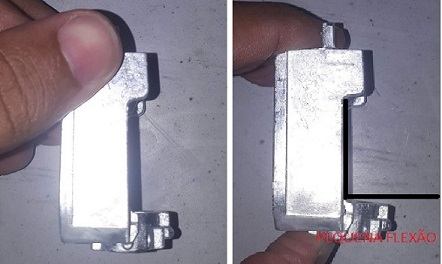
\includegraphics{Textuais/Images/garfo.jpg}
    \caption{Exemplo de deformação ocorrida durante o processo de fabricação em comparação com produto aprovado}
    \label{fig:my_label}
\end{figure}



% ----------------------------------------------------------
% Fim Arquivo